% Draft: test results of the 7-day trajectory models (LSTM vs GRU), manual segment, calendar cutoff.
% Source: workshops/w2/artifacts/sherlock_w2_manual_c14_traj/comparison/*.csv (March test, 113,870 users).
% Figures: docs/w2/figures/traj_*.png, copied from that folder (section 5.3 of w2_trajectory_models.ipynb).

\subsection{Trajectory Models: Test Results}

Both models were refitted on all of February and predict days 83--89 of the March window once.
Every target is compared with a predictor that learns nothing (Table~\ref{tab:traj-events}).

\begin{table}[htbp]
\centering
\caption{Event targets on the March test set. Daily targets are scored per user-day; weekly payment per user.}
\label{tab:traj-events}
\begin{tabular}{llrrrr}
\toprule
Target (prevalence) & Predictor & AUC & AP & Brier & Mean $\hat p$ \\
\midrule
\texttt{active} (0.664)      & LSTM            & 0.803 & 0.885 & 0.168 & 0.623 \\
                             & GRU             & \textbf{0.808} & \textbf{0.888} & \textbf{0.164} & 0.651 \\
                             & mean of days 76--82 & 0.769 & 0.839 & -- & -- \\
                             & persistence     & 0.685 & 0.762 & -- & -- \\
\midrule
\texttt{pay}, daily (0.025)  & LSTM            & \textbf{0.902} & \textbf{0.185} & 0.022 & 0.023 \\
                             & GRU             & 0.892 & 0.175 & 0.022 & 0.024 \\
                             & expiry rule     & 0.692 & 0.111 & -- & -- \\
\midrule
\texttt{pay}, weekly (0.170) & LSTM            & 0.979 & 0.903 & 0.046 & 0.120 \\
                             & GRU             & \textbf{0.980} & \textbf{0.903} & \textbf{0.043} & 0.124 \\
                             & expiry rule     & 0.714 & 0.585 & -- & -- \\
\bottomrule
\end{tabular}
\end{table}

\paragraph{Events are predicted well.}
Whether a user listens on a given day is ranked with AUC 0.81, against 0.77 for the share of active
days in the previous week, and the mean predicted probability (0.65) matches the observed rate (0.66).
Payments are where the model adds the most: it identifies who pays during the week with AUC 0.98 and
AP 0.90, against 0.58 for a rule that expects every customer to pay on their expiry date. The daily AP
is lower (0.18, still 7.5 times the 2.5\,\% prevalence) because the model knows \emph{who} will pay
much better than \emph{on which day}. Figure~\ref{fig:pay-expiry} aligns every forecast day to the
expiry known on day 82: manual customers pay mostly on the day \emph{after} the expiry (37\,\% of
them, against 12\,\% on the expiry day), which is why a rule that bets on the expiry day itself does
poorly. Both models learned this peak and its tail of late payments, but spread it over the
neighbouring days (24--29\,\% predicted on day $+1$, 19--22\,\% on day 0).

\paragraph{Calibration.}
\texttt{active} is well calibrated (Figure~\ref{fig:event-calibration}). Daily payment probabilities
are right on average (0.024 vs 0.025) but too flat: the highest-risk days are over-predicted and the
rest under-predicted, the same smearing seen in Figure~\ref{fig:pay-expiry}. Combined as seven
independent days they underestimate the weekly rate (0.12 vs 0.17; users given 0.7 actually pay
93\,\% of the time), so a simulator should draw at most one payment per week, with the day taken from
the normalised daily probabilities, rather than seven independent draws.

\paragraph{Listening amounts are not.}
The point forecast of listening is $p(\text{active}) \times \text{amount if active}$. Its MAE in
$\log(1+x)$ units is 1.010 (GRU) and 1.027 (LSTM): 5\,\% better than repeating the last day, but
slightly worse than the mean of the last seven days (0.986). The model's RMSE is lower than every
baseline (1.57 vs 1.70), i.e.\ it avoids large errors, but under absolute error a smooth average is
the best any predictor can do. This is also why the example trajectories look poor: an expected value
lies between ``silent'' and ``listening'', a level a real user never shows on a single day.
Users who were silent for weeks and come back, or who stop abruptly, cannot be anticipated from
their history by any of the predictors.

\paragraph{Paid amount.}
On real payment days the predicted amount is worse than the last amount paid (MAE 53--61 NTD vs
33 NTD; plan days 8.3--9.4 vs 7.6). The simulator should reuse the last plan instead of this head.

\paragraph{LSTM vs GRU.}
The GRU has a lower per-user listening MAE (paired bootstrap difference 0.017, 95\,\% CI
[0.0168, 0.0178]), a better \texttt{active} AUC and the same weekly payment AP, with half the
parameters (45k vs 92k) and 34\,\% less time per epoch. The LSTM is marginally better on the daily
payment AP (0.185 vs 0.175). The GRU is kept.

\begin{figure}[htbp]
  \centering
  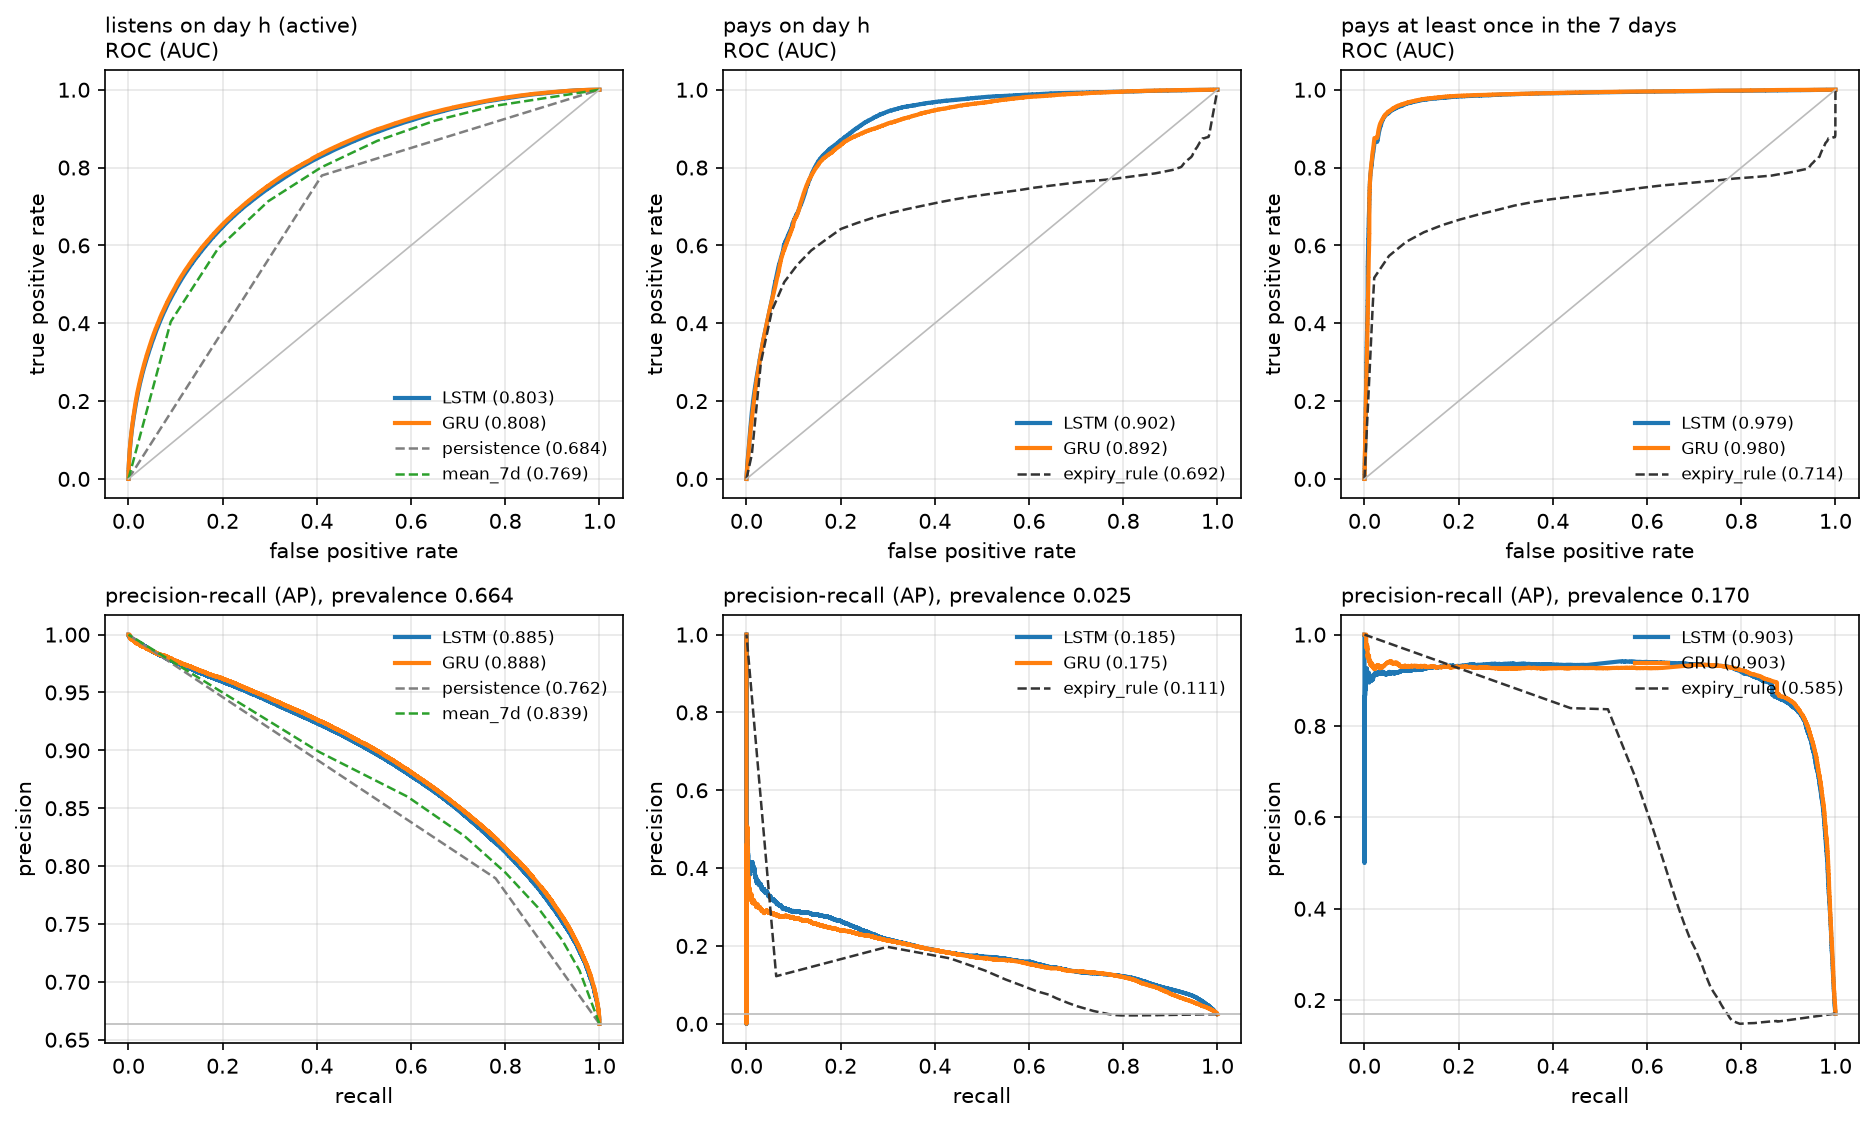
\includegraphics[width=\linewidth]{figures/traj_event_curves.png}
  \caption{ROC and precision-recall curves of the event targets on the March test set, against the baselines.}
  \label{fig:event-curves}
\end{figure}

\begin{figure}[htbp]
  \centering
  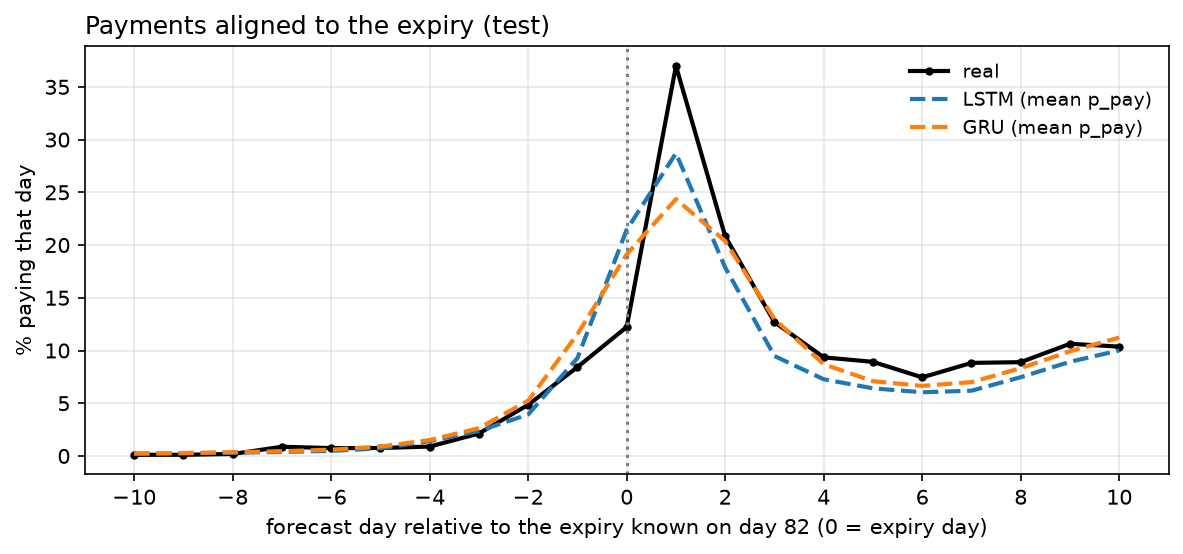
\includegraphics[width=0.8\linewidth]{figures/traj_pay_by_expiry.png}
  \caption{Daily payment rate aligned to each user's expiry (known on day 82): real vs mean predicted probability.}
  \label{fig:pay-expiry}
\end{figure}

\begin{figure}[htbp]
  \centering
  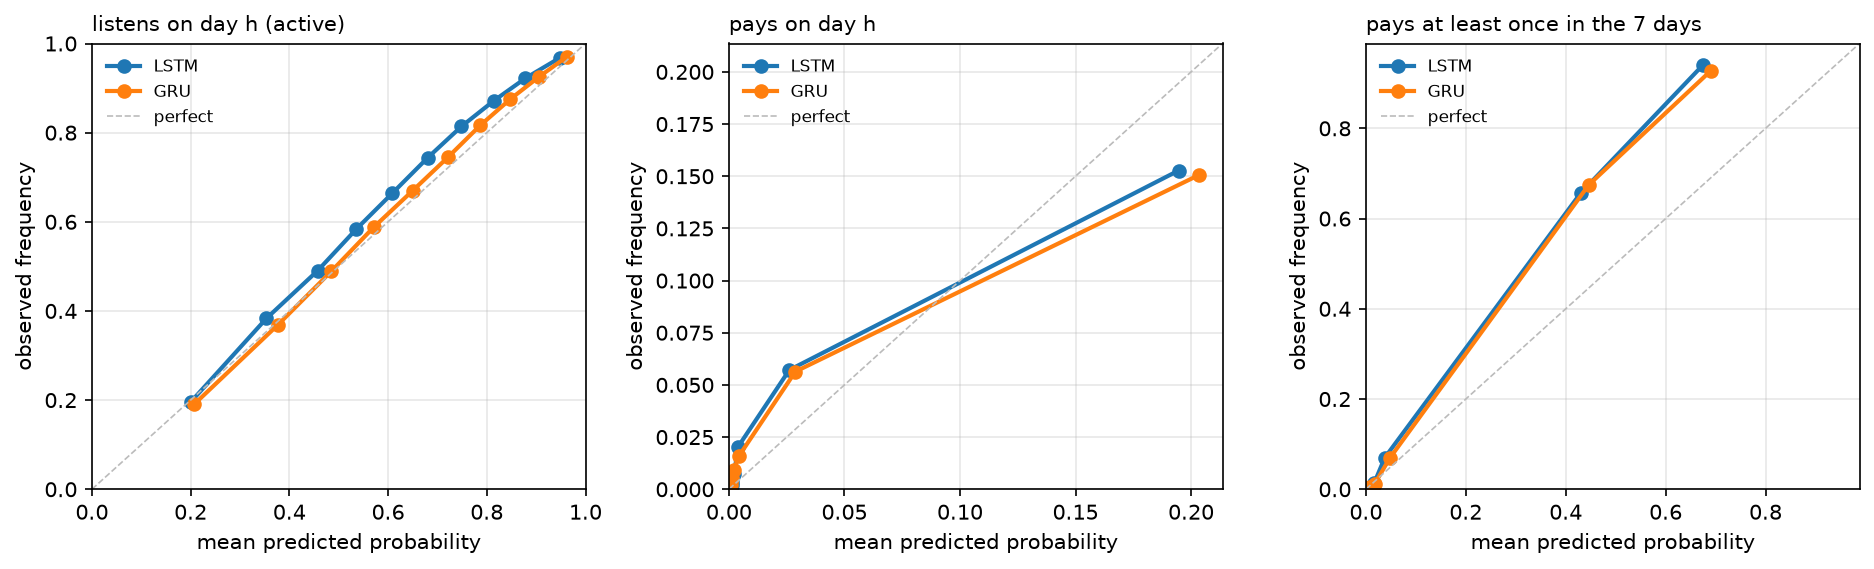
\includegraphics[width=\linewidth]{figures/traj_event_calibration.png}
  \caption{Calibration of the event probabilities (deciles of the predicted probability).}
  \label{fig:event-calibration}
\end{figure}

\begin{figure}[htbp]
  \centering
  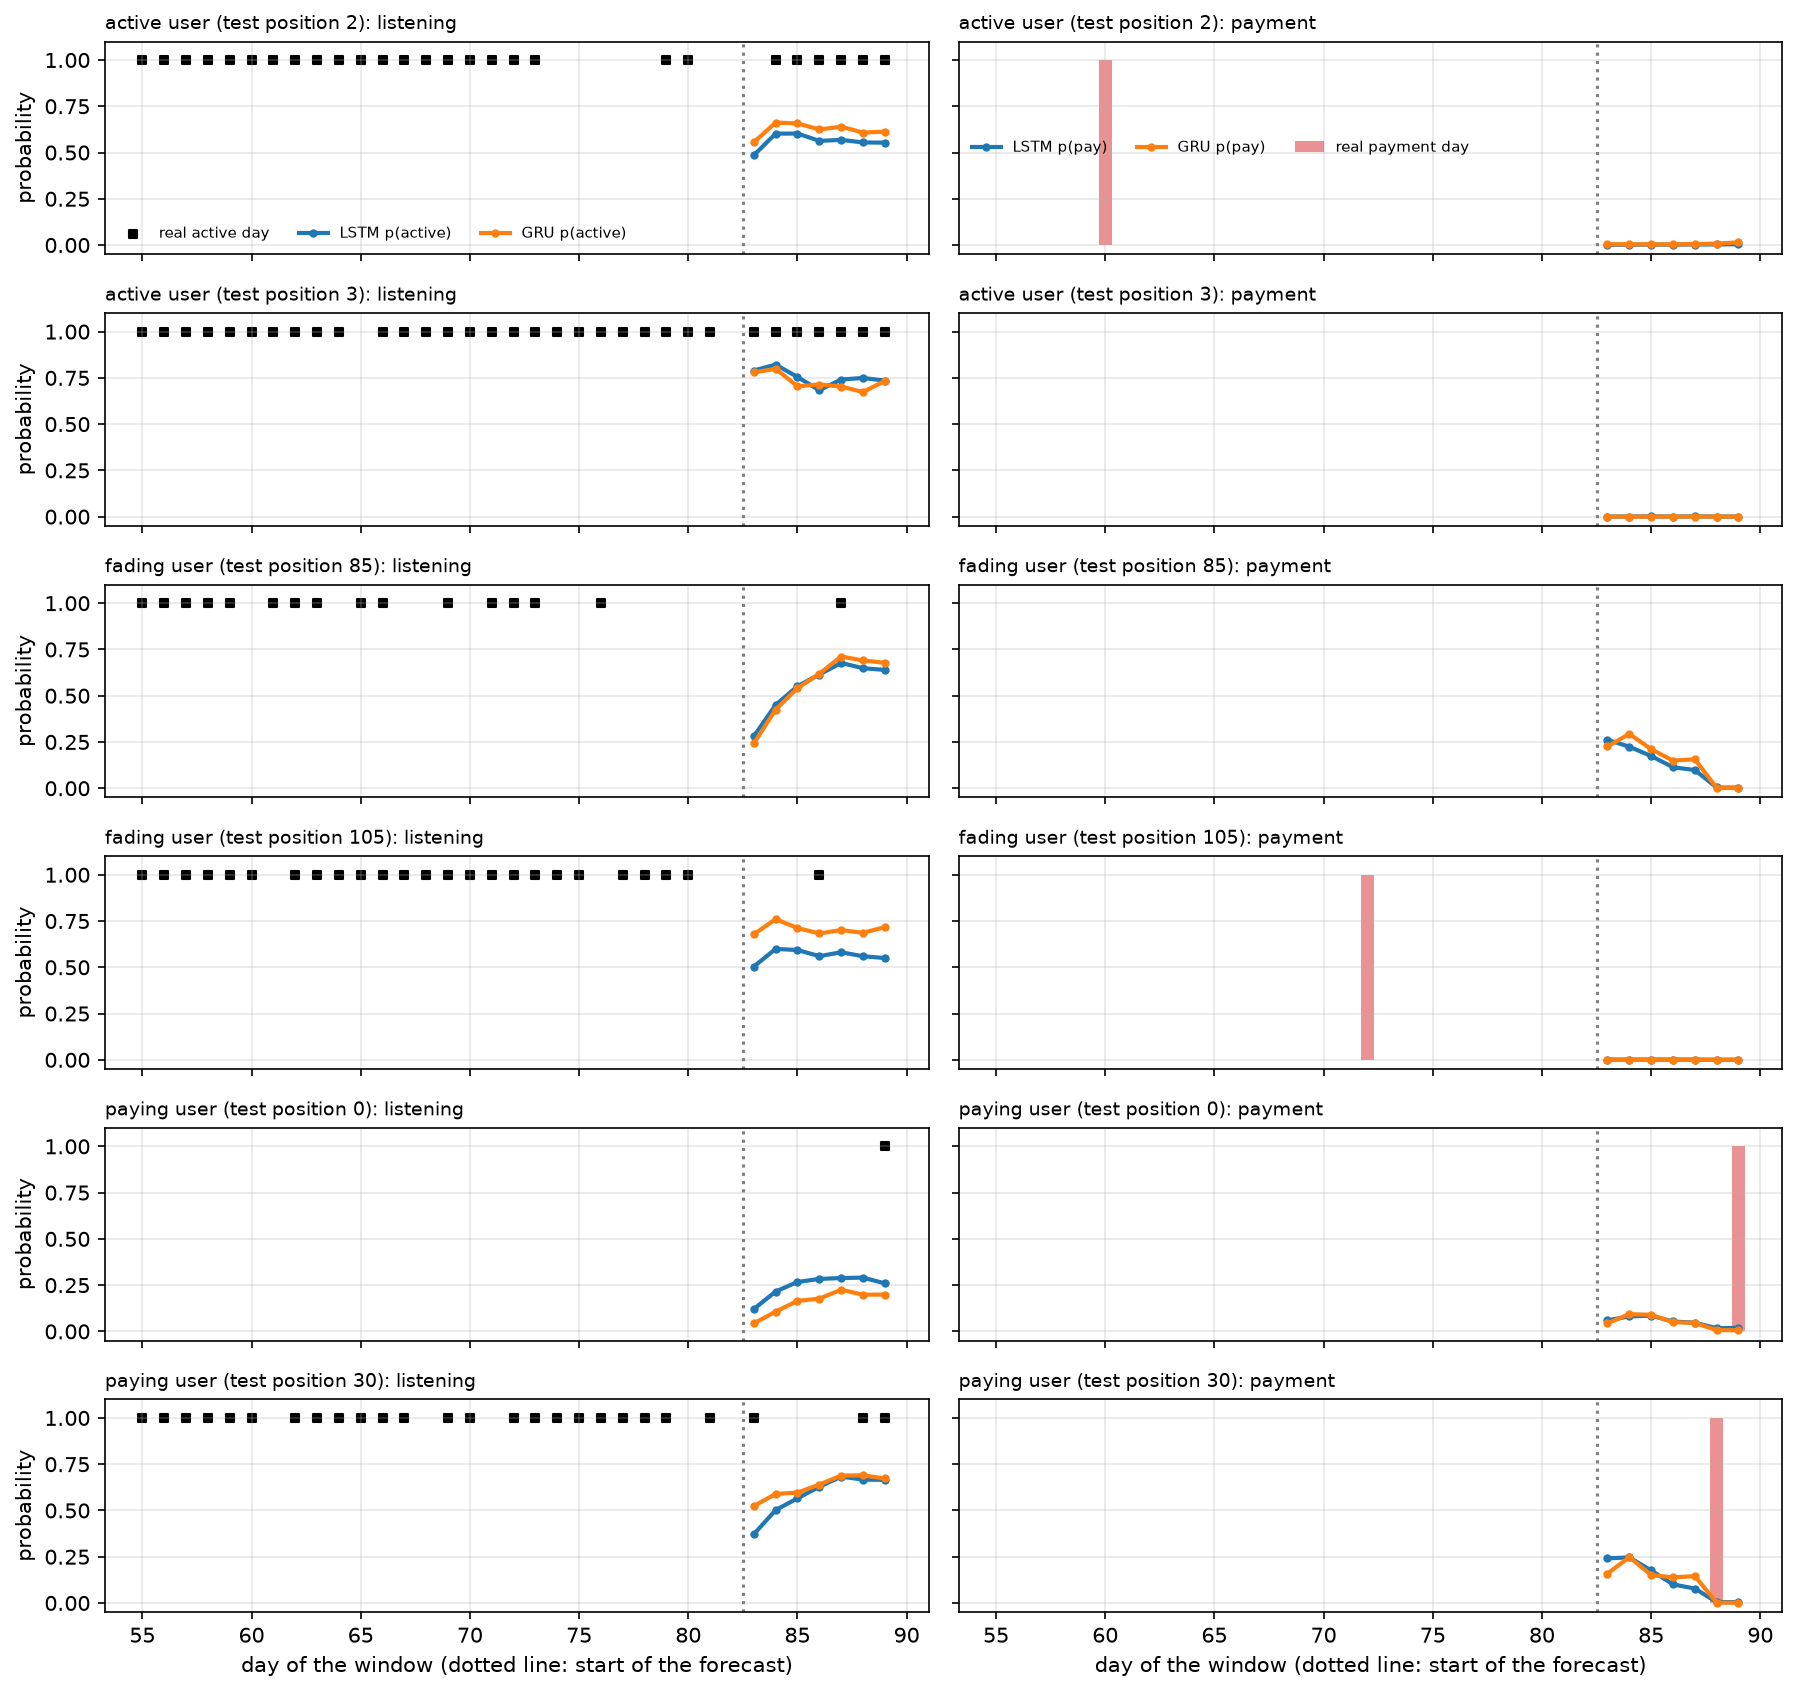
\includegraphics[width=\linewidth]{figures/traj_example_events.png}
  \caption{Example users: real active and payment days against the predicted probabilities.}
  \label{fig:example-events}
\end{figure}
